In this chapter it will be showcased how the \emph{Hybrid Place-, Place as Dialogue- and Sense-making strategies} have been operationalised as a theoretical lens to form a proposal of how one can design for meaningfulness. 

This chapter presents the thoughts behind and making of this thesis research contribution: \emph{the framework}.

\section{14 dialogical principles}

The initial problem framing was concerned with designing an installation that addresses sustainability, which triggered a design process and conceptual exploration of sustainability-themes worthy of investigation. Guided by this framing I chose to explore \emph{the relationship between human and nature}. Through literature review (Chapter 2), essay-writings (see appendix) and prototyping (see Chapter 8: Exploring input through plants) I learned that elements, or qualities, (I tend to use the two terms litt hipp som happ). 


Main RQ: How can one design meaningful interactive experiences in
a museum space that addresses sustainability?
answered by: (Sub-RQ): synthesising (or objectifying?) meaningful-
ness as a quality that you can design for in a museum.
through: (Sub-RQ): finding/identifying dialogic relations between
visitor and installation.

Need to defend and justify \emph{why} meaningfulness. 

\begin{figure}[H]
\centering 
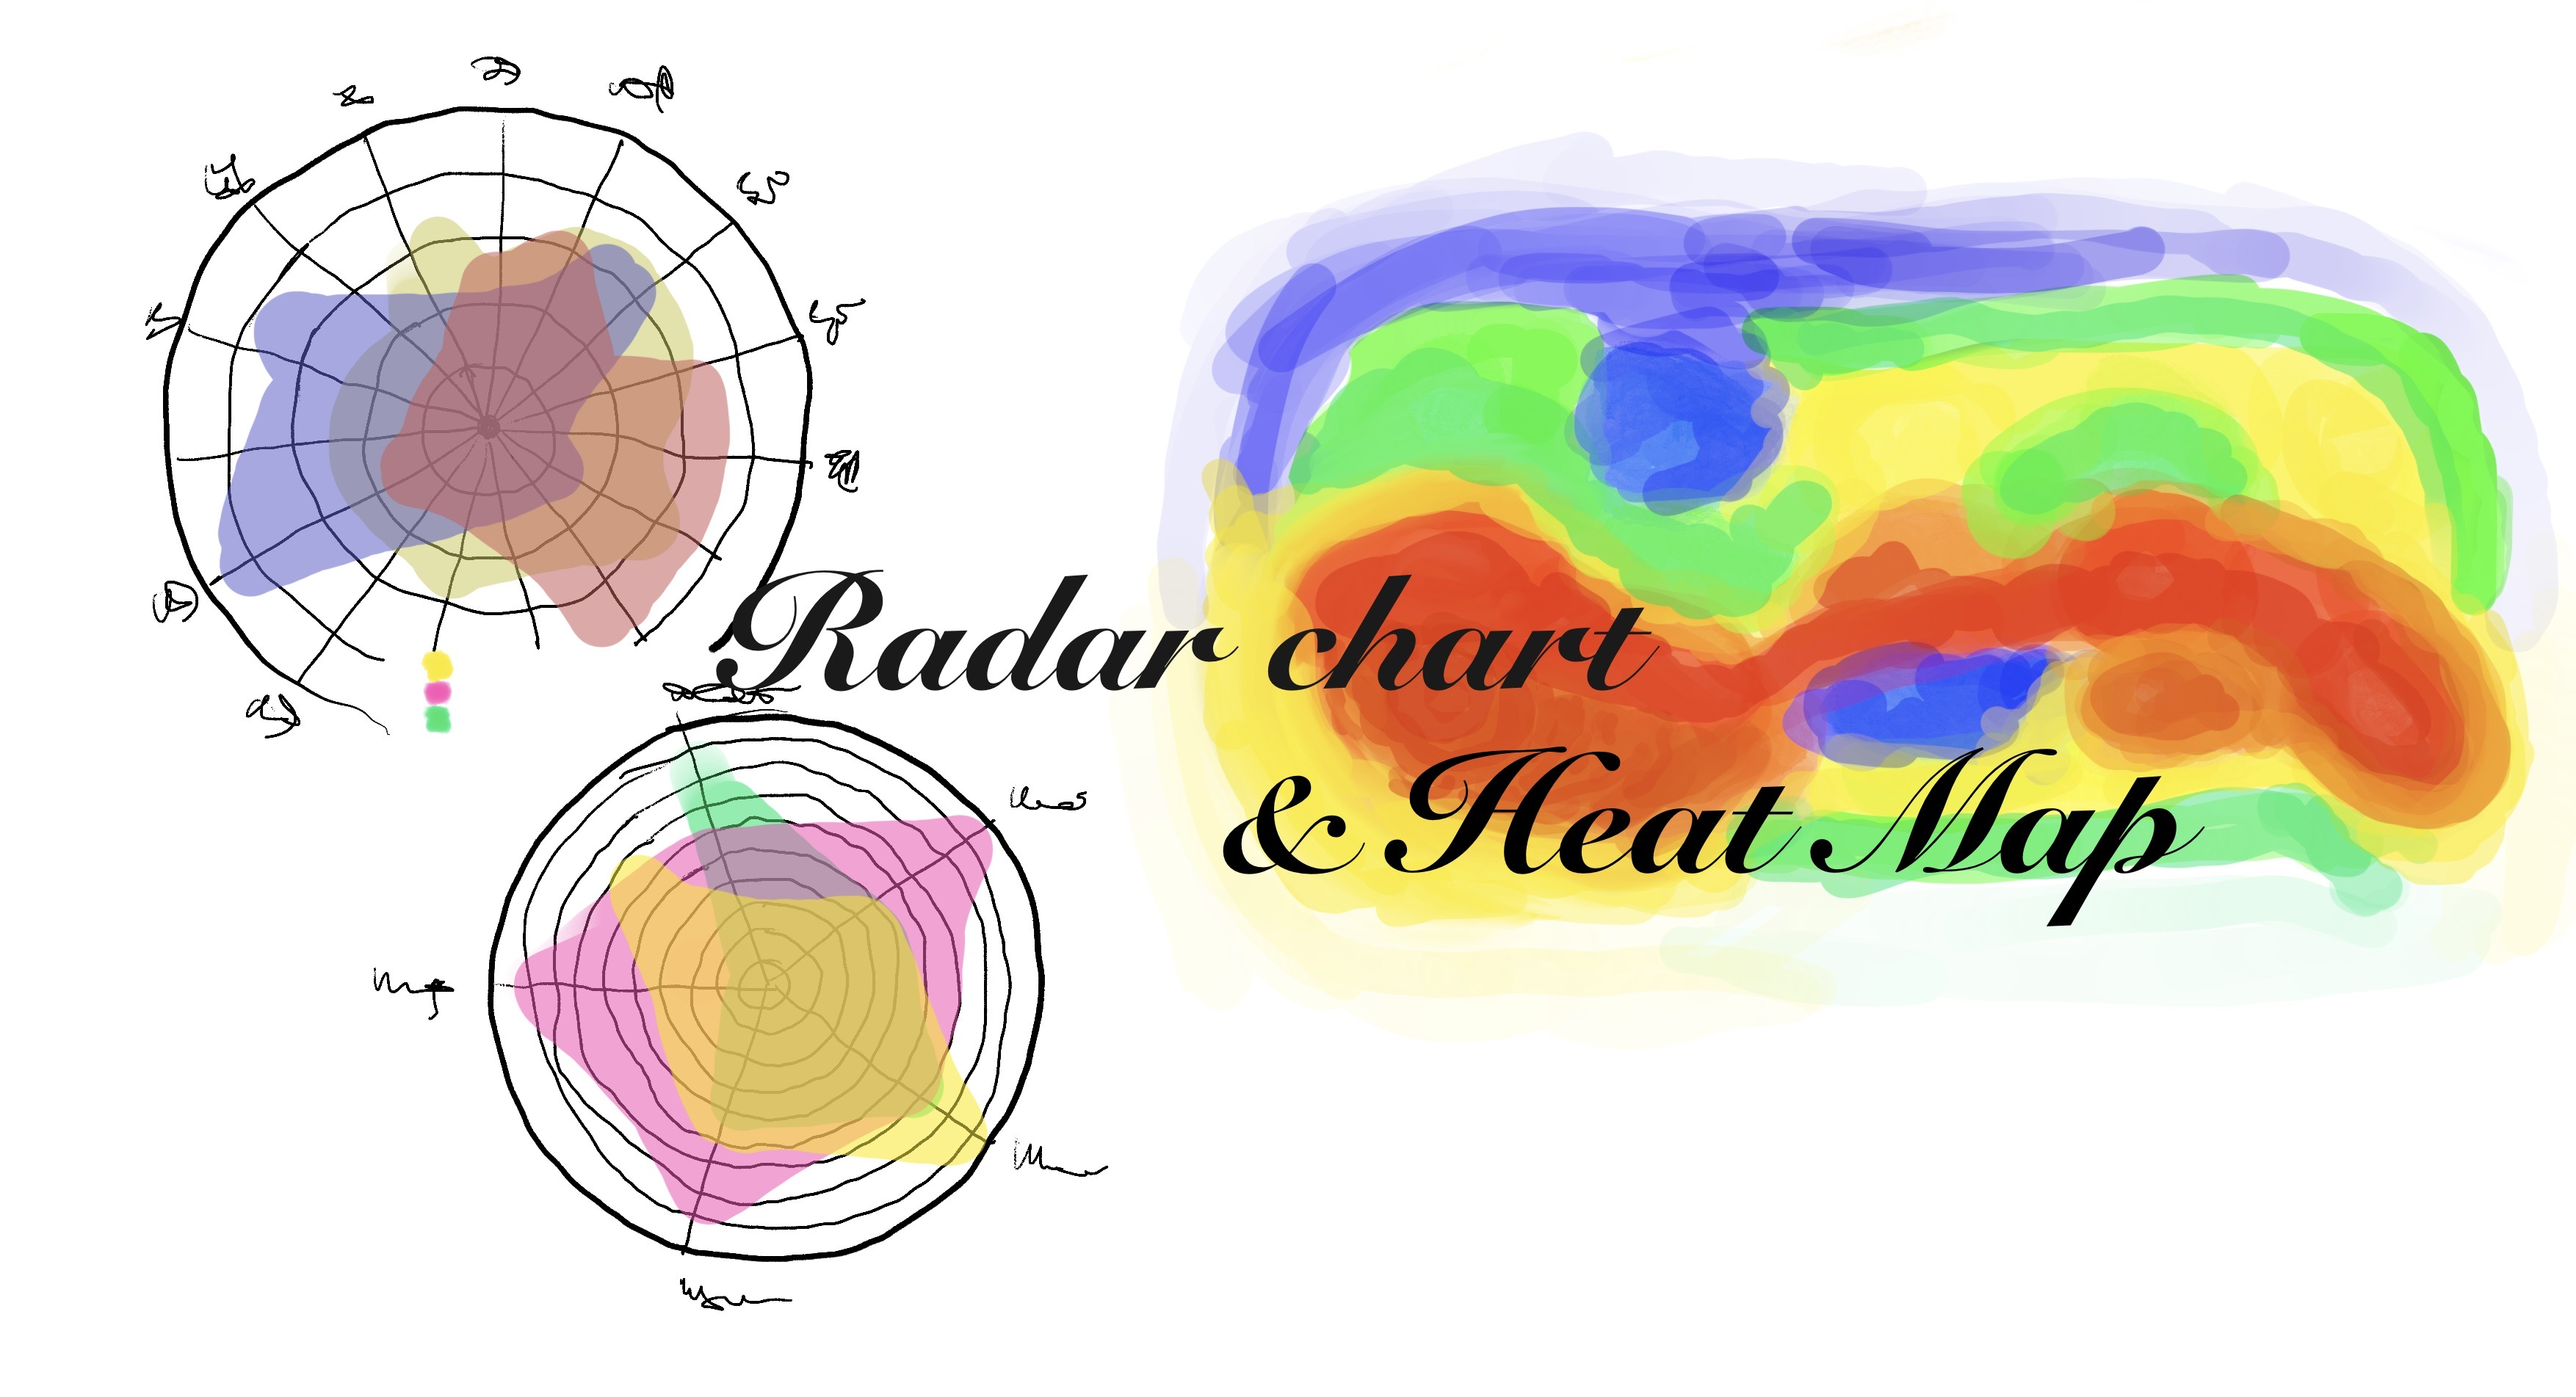
\includegraphics[width=10cm]{pictures/Theory/radar_and_heatmap.jpeg}
\caption{}
\end{figure}


\section{Design for interactive meaningful experiences in a museum}

The main purpose of this analysis-oriented part is to contribute with knowledge that make visible dialogic qualities between interactive installations and visitor-experience. 

"Finally, by making different things intended to address the same problematic situation, RtD can reveal design patterns \autocite{Alexander_book} around problem framings, around specific interactions, and around how theory can be operationalized" \autocite[p. 178]{zimmerman_research_2014}.


"Each one of these patterns is a morphological law, which established a set of relationships in space, which can always be expressed in the same general form: $X \rightarrow r (A, B, ...)$, which means: Within a context of type X, the Parts A, B, ... are related by the relationship r." \autocite[p. 90]{Alexander_book}.


The way I understand meaningfulness is to compare three approaches; how do the installation fit into the museum agenda? How well does the installation disseminate the message conveyed? and then, in what degree is the interactive elements in the installation dialogic (e.g. how well do they stimulate conversation). In my search for how one can design meaningful interactive experiences in a museum space that addresses sustainability, I propose the theoretical lens I have used to understand and look for meaningfulness in museums. This visualisation illustrates three "edges", of what I mean when I talk about (and synthesise) meaningfulness. 


\begin{figure}[h]
\centering 
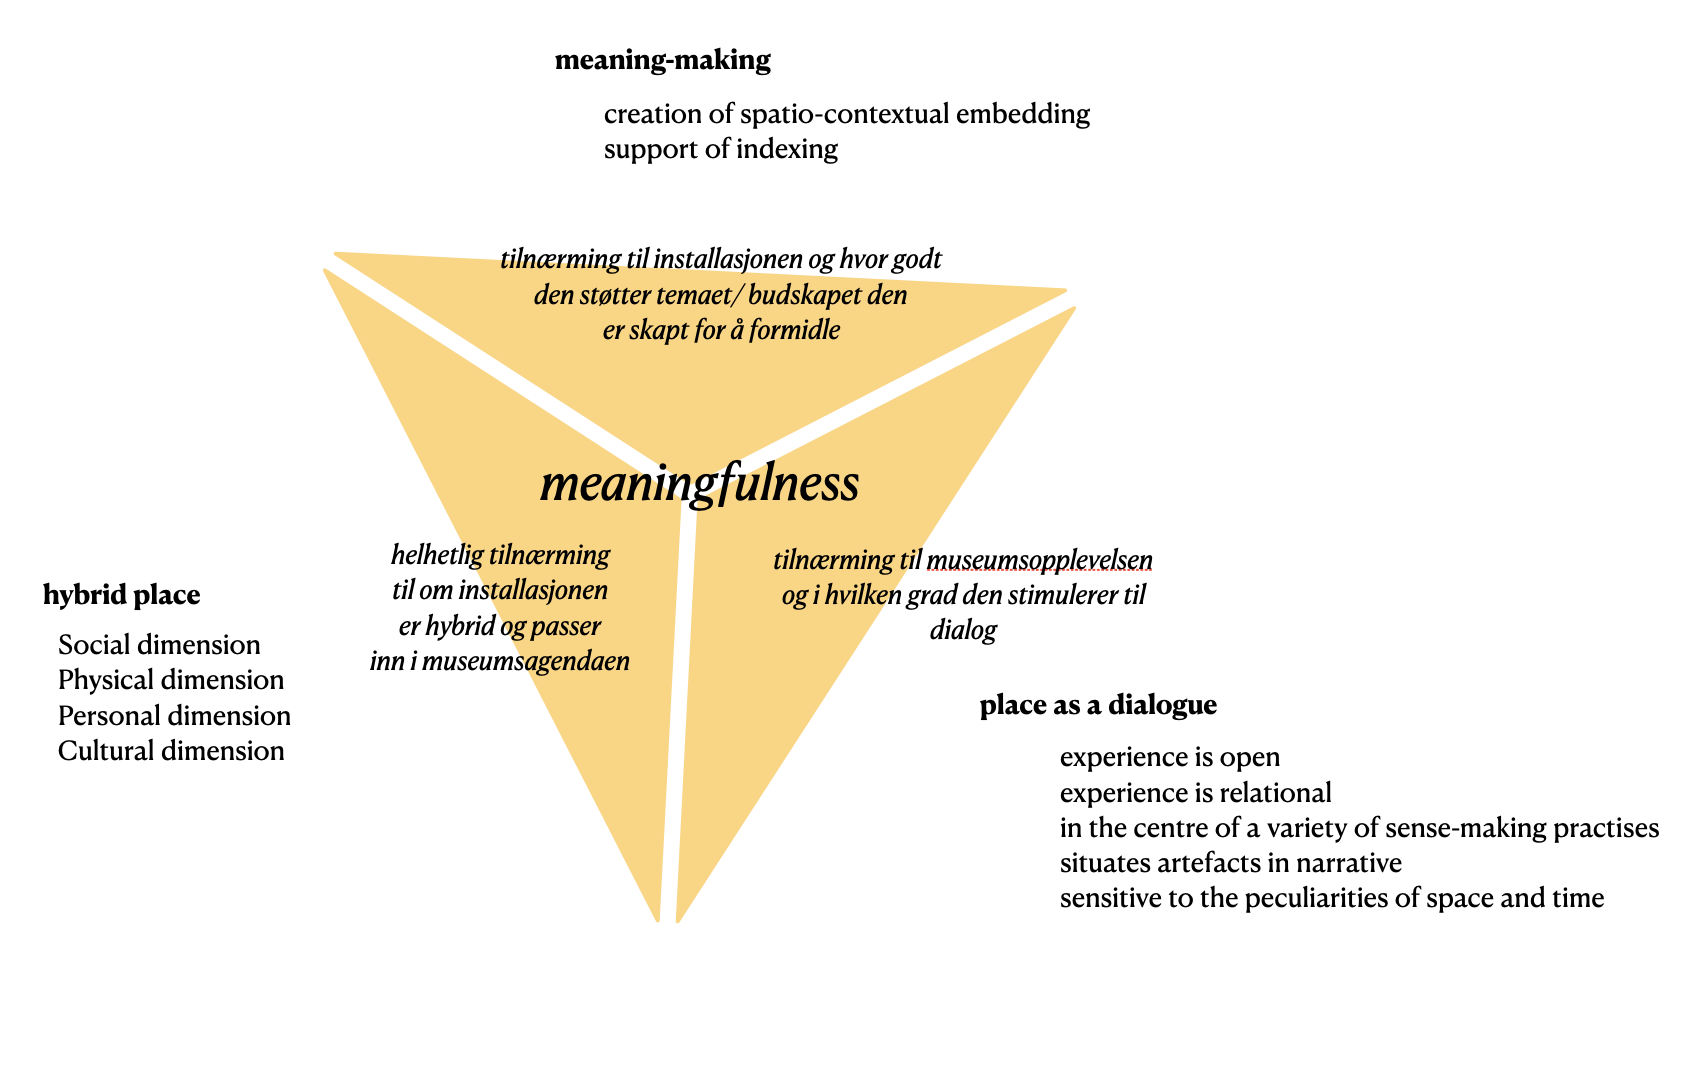
\includegraphics[width=13cm]{pictures/meaningfullness_triangle.png}
\caption{}
\end{figure}


\begin{figure}[h]
\centering 
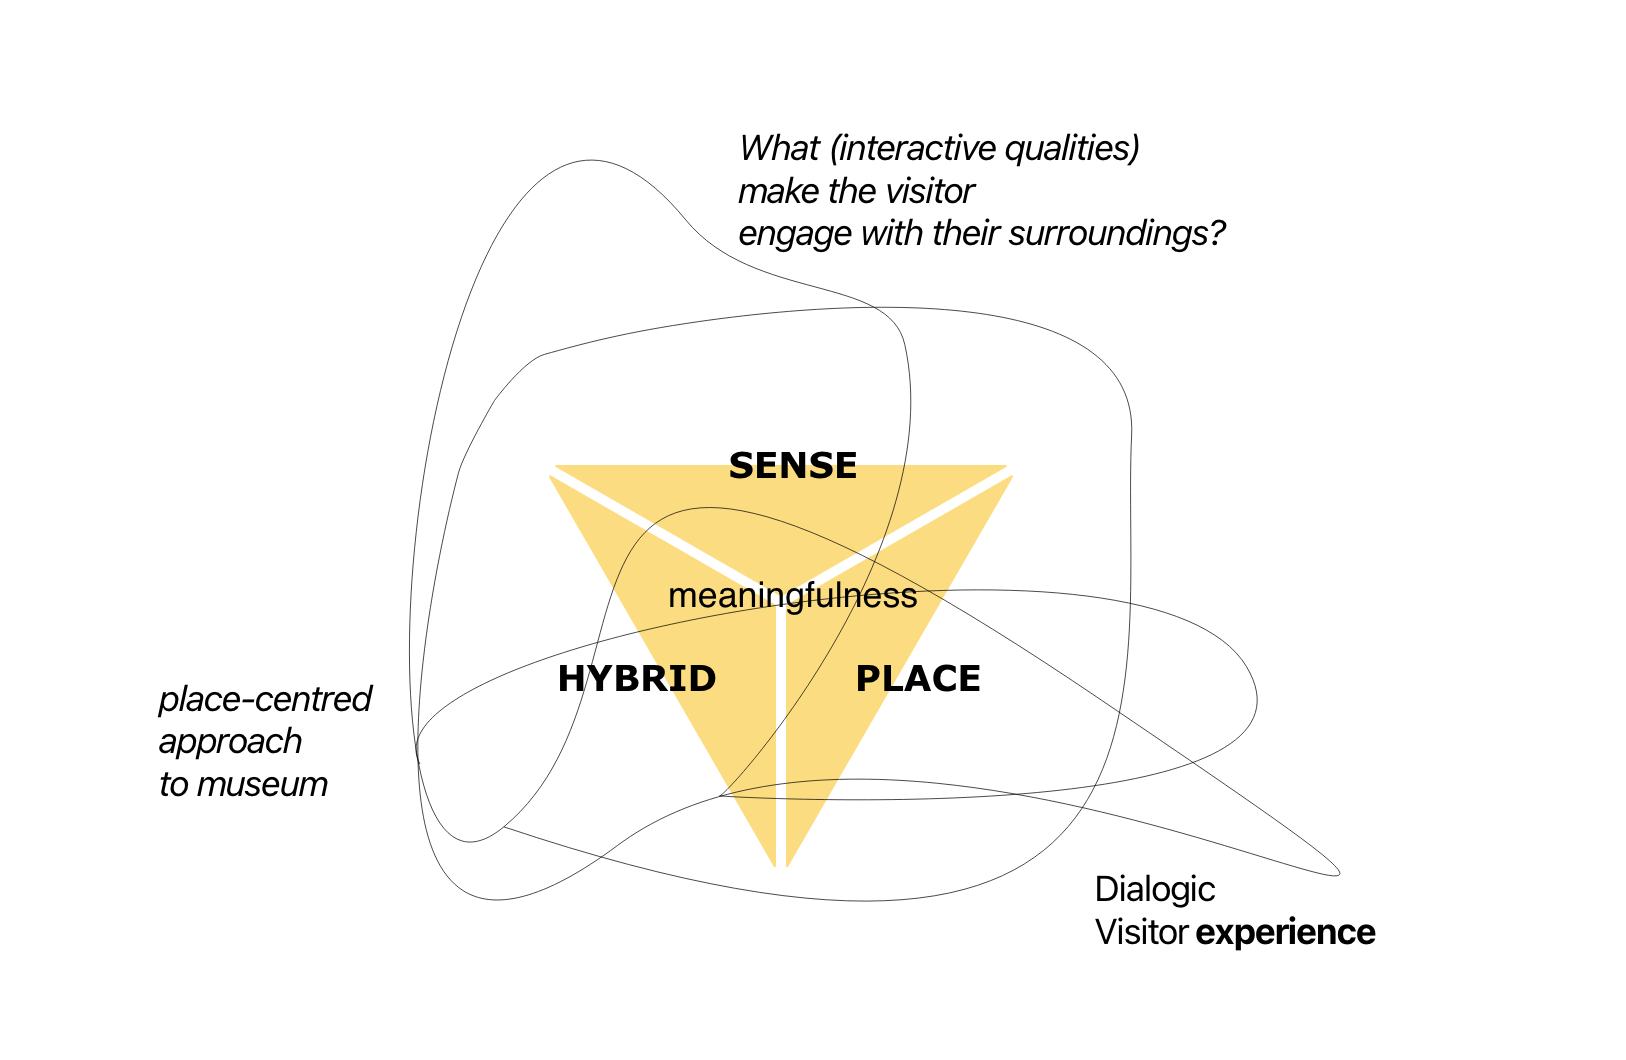
\includegraphics[width=13cm]{pictures/Theory/early_iteration_framework.png}
\caption{}
\end{figure}

\begin{figure}[h]
\centering 
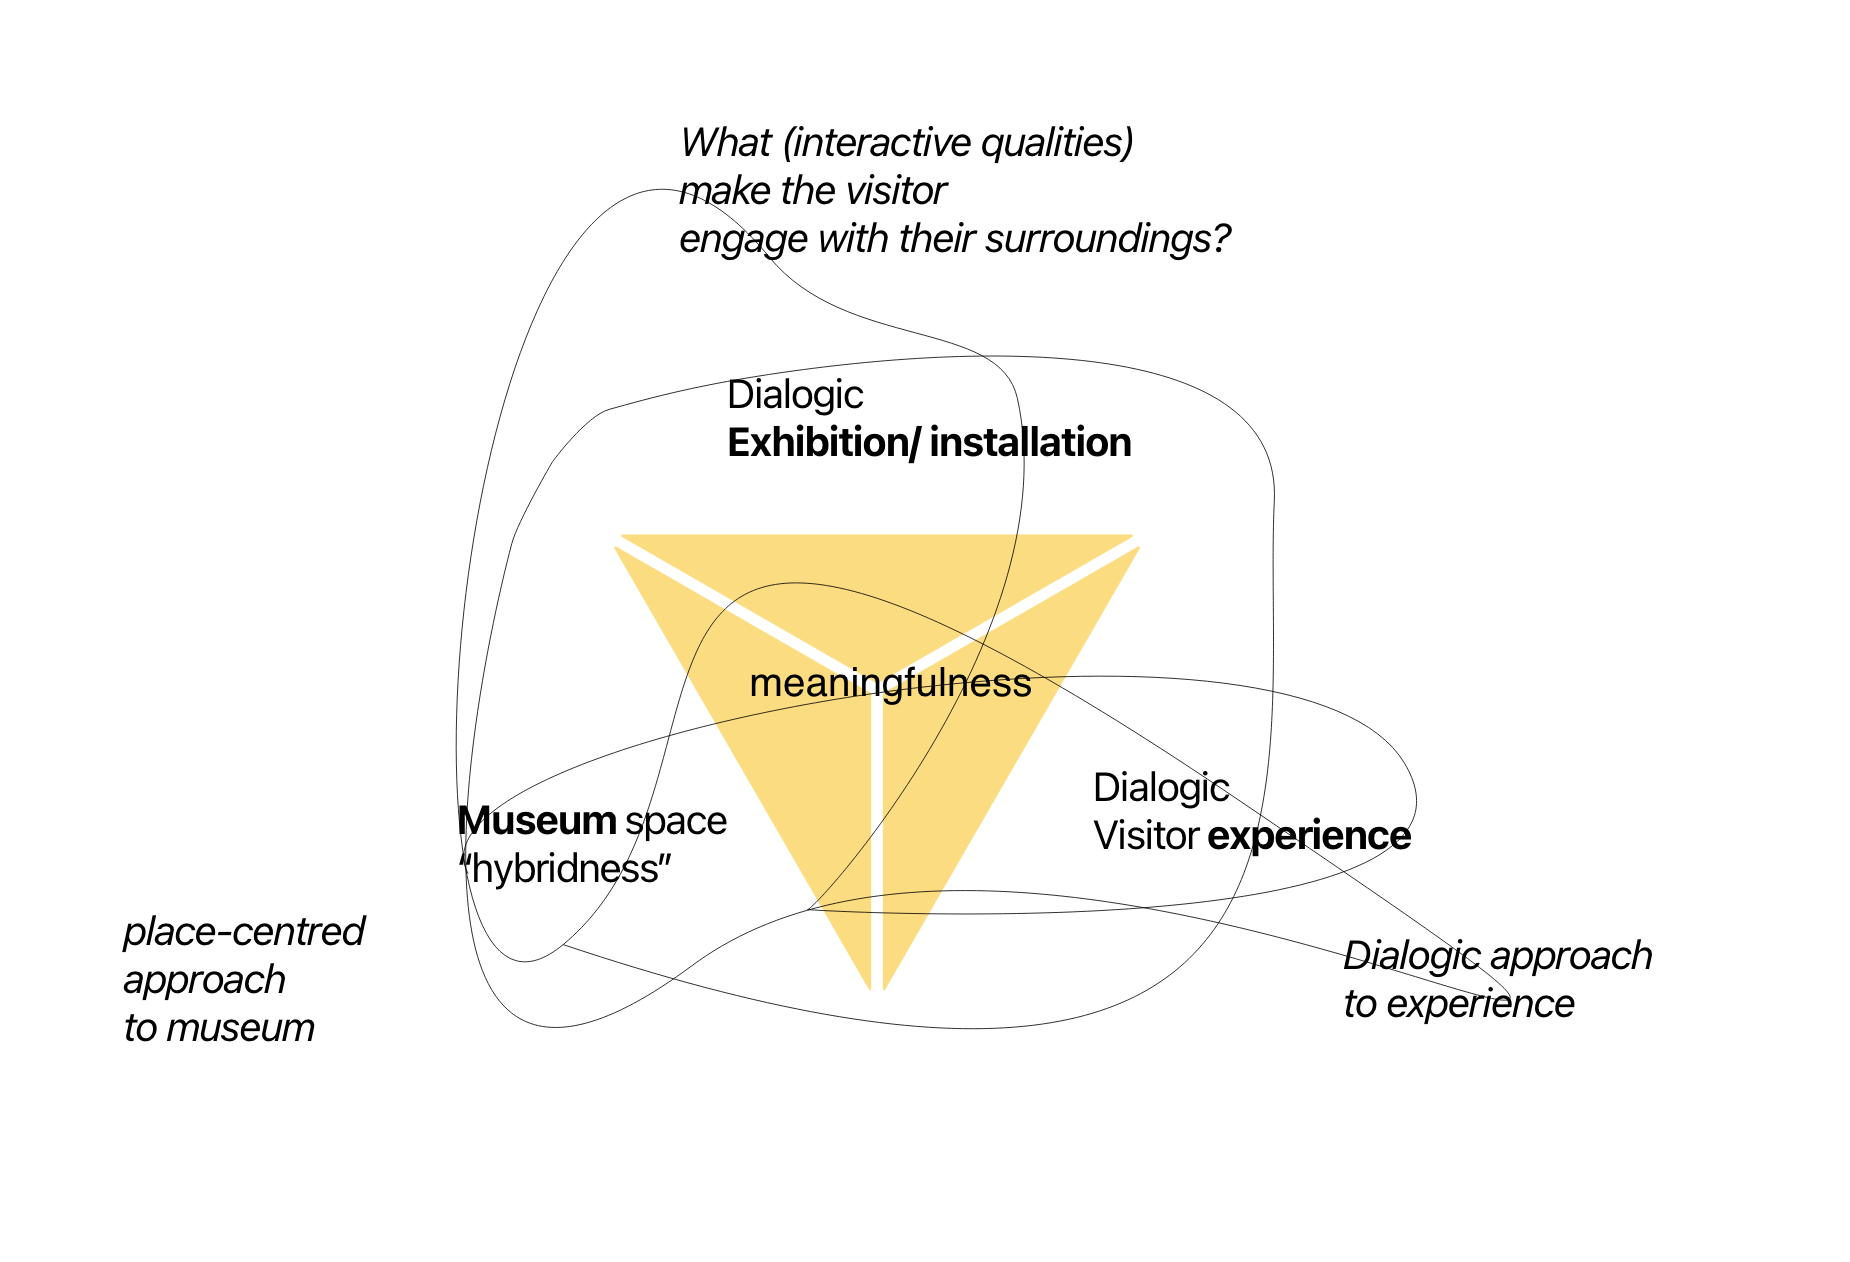
\includegraphics[width=13cm]{pictures/Theory/meaningfulness_triangle.png}
\caption{}
\end{figure}

The visualisation illustrates my definition of meaningfulness as a quality that you can design for. The triangle is an attempt to showcase what "aspects" I borrow/build upon from each respective theoretical framework, and then how together they fulfill three dimensions to how meaningfulness can be understood (interpreted?).
From the Hybrid Place framework I borrow four dimensions; the \emph{physical, social, personal and cultural}, as a way to portray/ map out the installation in relation to its environments. I see it as a holistic approach to judge the "hybridness" of the installation in relation to its surrounds, so that I can see in what dimensional direction the potential meaningful relation between visitor and installation could be.

The practical application of this analytical tool is something like this (the tables underneath), where I have plotted in the different installations and exhibitions to their respective tables. A thoruough walkthrough of the analysis is accounted for in Chapter 9: Analysis.
